\section{Protocol}
\label{sec:protocol}

We propose two settings for secure publish-process-subscribe protocols :
(\emph{i.}) with an honest-but-curious external entity in addition to standard
publish-subscribe entities, publishers, subscribers, and a broker, as shown in
Figure~\ref{fig:pps-out} and (\emph{ii.}) without such an external entity as
shown in Figure~\ref{fig:pps-local}. First setting is suitable for less
resourceful devices, such as, mobile phones, and the second setting is suitable
for large organiazations with hundreds of subscribers. We describe our protocol
and system in first setting, but they could be easily adapted to the second
setting.

\begin{figure}[h]
	\centering
	
		\begin{subfigure}{0.45\textwidth}
		\centering
		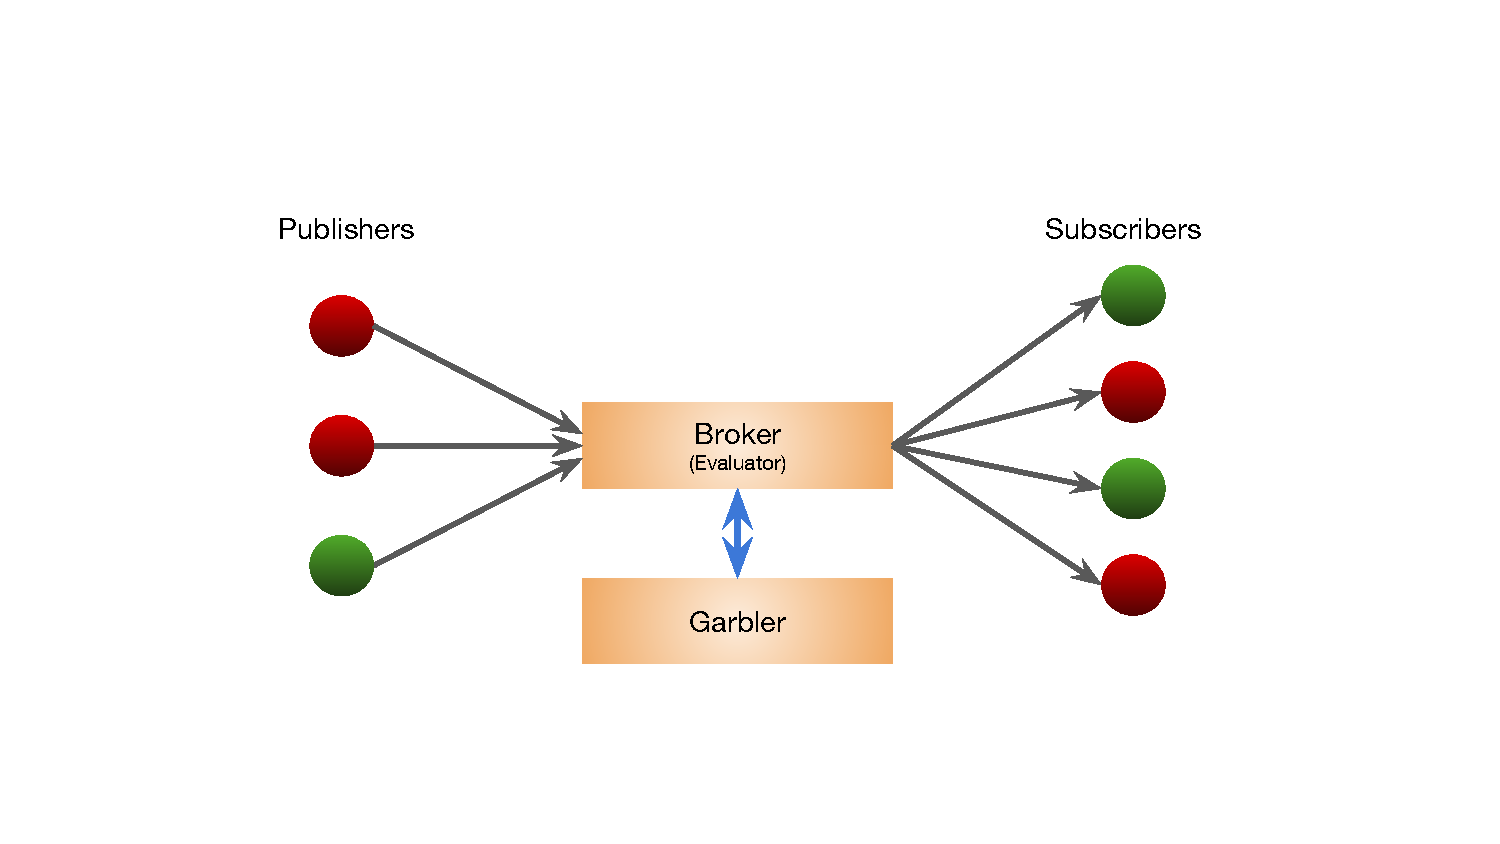
\includegraphics[width=0.7\textwidth]{figures/pps-out}

		\caption{Publish-Process-Subscribe setting with a separate entity,
		\garbler, to avoid expensive processing and communication at the
		subscriber's end. This is suitable for mobile devices. We describe our
			protocol and system in this setting. 
		}

		\vspace{12pt}
		\label{fig:pps-out}
	\end{subfigure}
	
	\begin{subfigure}{0.45\textwidth}
		\centering
		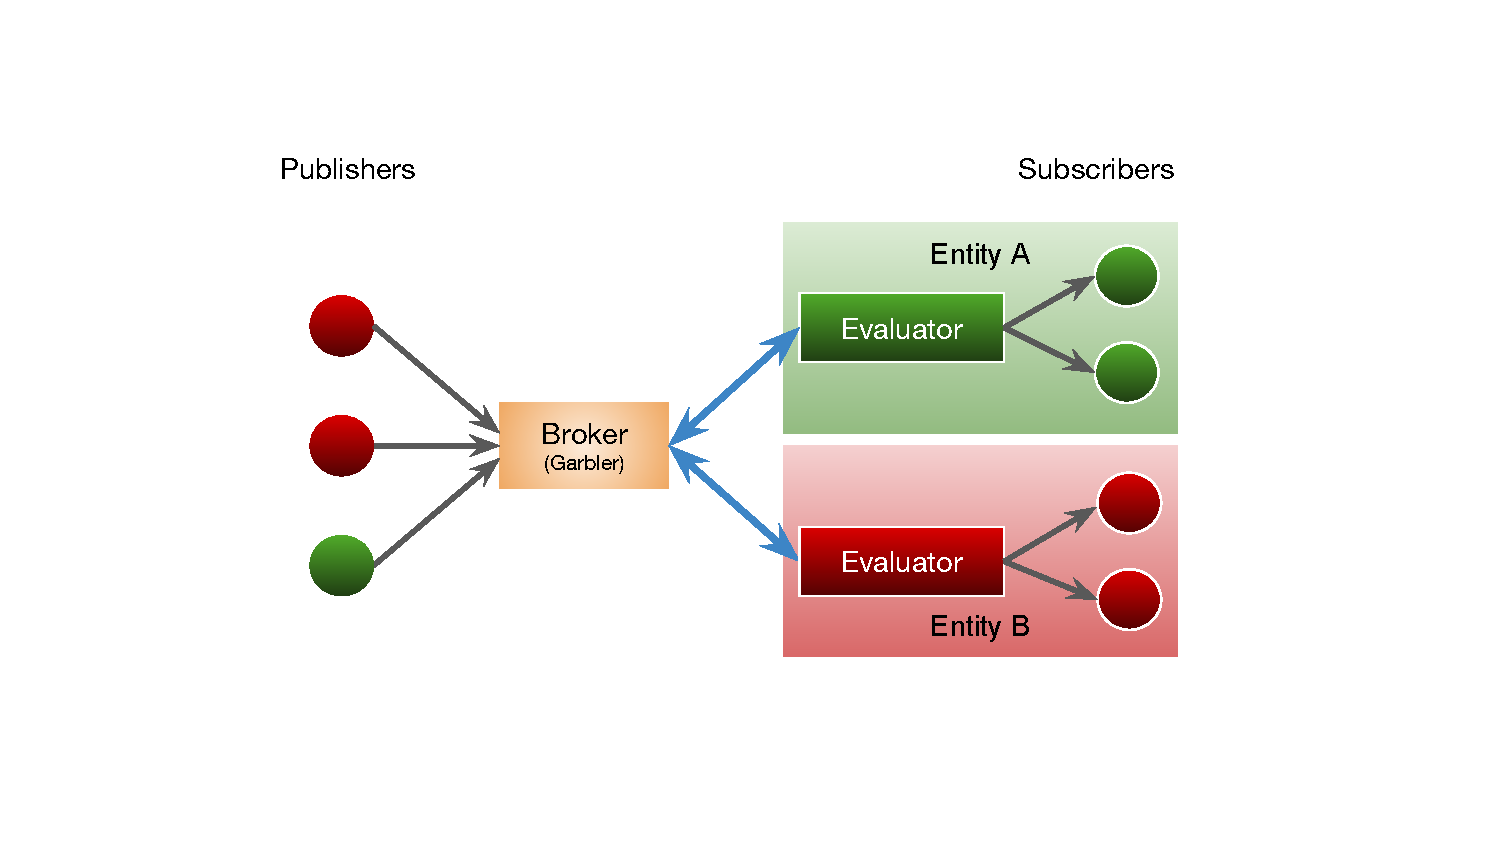
\includegraphics[width=0.7\textwidth]{figures/pps-local}

		\caption{Publish-Process-Subscribe setting with only a \broker, just like
		traditional topic-based publish-subscribe systems. This is suitable for
		large organizations, with hundreds of subscribers, who can set up local
		computation. While we describe our protocol and system in the setting of
		Figure~\ref{fig:pps-out}, they can be easily adapted to this setting.}

		\label{fig:pps-local}
	\end{subfigure}


	\vspace{12pt}
	\caption{Publish-Process-Subscribe System's Architecture. {\color{red}Red} shows {\color{red}malicious} and {\color{green} green} shows {\color{green} honest} entities.
			}
	\label{fig:pps}
\end{figure}

\iffalse

The subscriber cannot compute it tehmselvds as they are using data from some
other entity, wihch may not want to share raw data.

\noindent\textbf{Publish-Subscribe}

\noindent\textbf{Garbled Circuits}

\noindent\textbf{Private-set-intersection (PSI)}

\fi




We describe a base secure publish-process-subscribe protocol first, for ease of
understanding and reasoning about security, followed by extensions for reducing
communication and efficiently handling malicious publishers disrupting the
computation.  We present a simulator for the base protocol to prove that a real
world adversary cannot do more harm then a simulator can do in the ideal world
(Definition~\ref{def:security}). We also describe security of extensions. We
describe our system in Section~\ref{sec:system}, which is not a mere
implementation of our protocol. We developed a range of system techniques, such
as, developing a new high-level functional language to describe computations
and generate circuits, extending garbled circuits library libgarble, identity
gates to make our protocol compatible with FreeXOR optimization, and establish
authenticated and encrypted channel on top of MQTT. 

We assume direct authenticated encrypted channels in this section.  However, in
our system, publishers and subscribers communicate directly only with \broker
and communicate indirectly with \garbler through \broker as showing in
Figure~\ref{fig:pps-out}. This allows us to implement our protocol on top of
MQTT.

\subsection{Base Protocol}
\begin{figure*}[h]
\begin{mdframed}[style=myframe]

\initialize
\begin{itemize}[leftmargin=18pt,itemsep=4pt,topsep=4pt]
 
	\item Each new publisher sends \broker a \policy specifying allowed
		computations on its data.

\end{itemize}

\subscribe
\begin{itemize}[leftmargin=18pt,itemsep=4pt,topsep=4pt]

	\item To subscribe computation $C$, subscriber sends a subscription request
		containing $C$ to \broker. If \broker allows subscriber to learn $C$'s
		output, it adds the subscriber to a list of $C$'s subscribers. 

\end{itemize}

\publish
\begin{itemize}[leftmargin=18pt,itemsep=4pt,topsep=4pt,after=]
		
	\item To publish $k$th value, publisher generates two pseudorandom wire
		labels, $w_0$ and $w_1$, for each bit of the value. 
		
	\item For each input bit $b$, publisher sends only $w_b$ to \broker and sends
		both $w_0$ and $w_1$ to \garbler.

\end{itemize}

\process
\begin{itemize}[leftmargin=18pt,itemsep=4pt,topsep=4pt]

	\item \broker waits for a specified time period $t$ to receive input wire
		labels, a single label $w_b$ for a bit $b$, from a subset of publishers
		$P_C$ whose policies allow $C$. After time period $t$, \broker sends
		\garbler identifiers of publishers in $P_C$ along with identifiers of
		publishers whose data wasn't received during time period $t$ and requests
		\garbler to garble circuit for $XOR \circ C$. $XOR$ is used to mask the
		output of the circuit.

	\item \broker sends \garbler the set of $C$'s subscribers $S_C$.
		
	\item \garbler generates a garbled circuit $GC$ for the circuit $XOR \circ C$
		using both wire labels for each input bit, $w_0$ and $w_1$ for a bit $b$,
		received from publishers in set $P_C$ hard-wiring nullifying value for
		publishers whose input labels weren't received by \broker as well as any
		publishers whose labels weren't received by \garbler. \garbler generates a
		random mask $r$ and use it to mask the output $o$ of $C$, such that
		evaluating $GC$ would result in a masked output $o+r$.
		
	\item \garbler sends $r$ to all subscribers in the set $S_C$ and $GC$ to
		\broker along with identifiers for publishers for which it hard-wired
		nullifying values.

	\item For every bit $b$ of the $C$ inputs, \garbler and \broker run a
		private-set-intersection-cardinality (PSI-C) protocol to determine wire
		labels consistency, i.e., if \broker input label for bit $b$, $w_b$, is one
		of the two \garbler labels for bit $b$, $w_0$ and $w_1$. If PSI-C outputs
		$1$, then the labels are consistent and if it's $0$ then the labels are
		inconsistent. \garbler will use nullifying values for inputs of all
		publishers with at least $1$ inconsistent wire label. 
		
	\item \broker evaluates the garbled circuit using wire labels sent by
		publishers in set $P_C$ ignoring labels for which \garbler hard-wired
		nullifying values, obtains masked output $o \xor r$, and sends $o \xor r$
		to all subscribers of computation $C$.
  
	\item Subscribers in the set $S_C$ use mask $r$ to unmask the output $o$.

\end{itemize}

\end{mdframed}
\caption{Base Protocol}
\label{fig:baseprotocol}
\end{figure*}


The base protocol uses direct communication with \garbler for ease of
explanation; publishers and subscribers in our system communicate with \garbler
only through \broker. This ensures compatibility with a standard topic-based
publish-subscribe system where publishers and subscribers communicate only
through \broker.

Each new publisher initializes by sending its \policy specifying allowed
computations on its data. To subscribe computation $C$, a subscriber sends a
subscription request to \broker.  To publish a value, publisher generates two
wire labels $w_0$ and $w_1$ for every bit $b$ of the value, sends both labels
$w_0$ and $w_1$ to \garbler, and only $w_b$ to \broker. \broker waits for a
specified time period to receive all input wire labels after which \broker
requests \garbler to garble the circuit for $XOR \circ C$.  A malicious
publisher can send inconsistent labels for a wire to \broker and \garbler,
e.g., $w_0$ and $w_1$ to \garbler and a random wire label $w_r$ to \broker.
Inconsistent labels prevent \garbler from correctly evaluating the garbled
circuit. We use private-set-intersection-cardinality (PSI-C) to determine
inconsistent labels. \garbler hard-wires nullifying values for publishers who
sent at least $1$ inconsistent label and publishers who didn't sent labels to
either \broker or \garbler. \garbler garbles the circuit such that evaluating
it outputs a masked output and send it to \broker.  Therefore, when \broker
evaluates the garbled circuit, it only learns a masked output, which it
forwards to $C$'s subscribers. \garbler sends the output mask to $C$'s
subscribers, who can then unmask the output.

\subsection{Security Proof of Base Protocol}
We describe a simulator \Sim that simulates the view of the \Adv in the real
world execution of our base protocol of Figure~\ref{fig:baseprotocol}. Our
security definition~\ref{def:security} and simulator \Sim ensures both
confidentiality and correctness.

The interesting case is when a subset of publishers are malicious and are
colluding with honest-but-curious \broker. \garbler is non-colluding
honest-but-curious. A malicious subscriber only receives output; it can only
reveal its own output, which is also possible in the ideal world execution.\\[6pt]
\noindent\textbf{Simulator.} \Sim receives from \F the number of publishers
$|P_C|$ whose policy allow computing $C$ on their data. \Sim creates $2l|P_C|$
random wire labels $(r_0^0, r_0^1), \ldots, (r_{2l|P_C|-1}^0
,r_{2l|P_C|-1}^1)$; $l$ being the bit-length of a publisher's input. We use
garbled circuit simulator $\Sim_{GC}$ as a blackbox; $\Sim_{GC}$ is the
simulator of the projective prv.sim secure garbling scheme with circuit $M
\circ C$ being the side information as described in~\cite{}. 

\Sim receives from \F $\F(M \circ C, \vec{x}_C)$, where $M$ is an XOR masking
function. \Sim sends $\F(M \circ C, \vec{x}_C)$ to $\Sim_{GC}$ and obtains a
fake garbled $GC_{fake}$. \Sim generates a random string $o_r$ of the same
length as output. \Sim sends $(GC_{fake}, r_0^0, \ldots, r_{2l|P_C|-1}^0, o_r)$
to \Adv. As garbled circuits distribution is independent of the input wire
labels, $GC_{fake}$ is computationally indistinguishable from the $GC$ in the
real execution. The random output $o_r$ in ideal execution is indistinguishable
from $o+r$ in the real execution.

In the ideal world, \Sim creates a fake garbled circuit $GC_{fake}$ that
doesn't use wire labels $(r_0^0, r_0^1), \ldots, (r_{2l|P_C|-1}^0
,r_{2l|P_C|-1}^1)$ for garbling. Otherwise, \Adv could use $r_0^0, \ldots,
r_{2l|P_C|-1}^0$ labels to evaluate the circuit on $0^{l|P_C|}$, which would
allow adversary to distinguish between real and ideal executions.

A malicious publisher can choose arbitrary wire labels in the real execution;
however, as long as the labels used in garbling are consistent with the labels
used for evluation, the honest subscriber output will be indistinguishable in
real and ideal executions. Our protocol ensures consistent wire labels.


\vspace{-8pt}
\subsection{Reduced Communication Extension}
\begin{figure}
\begin{mdframed}[style=myframe]

\initialize
\begin{itemize}[leftmargin=*,itemsep=2pt,topsep=2pt]
 
	\item Each new publisher generates and sends to \garbler a truly random seed
		$s$. This seed will be used to create wire labels without interaction.

\end{itemize}

\subscribe
\begin{itemize}[leftmargin=*,itemsep=2pt,topsep=2pt]

	\item In addition to registering subscription with \broker, subscribers for a
		computation $C$ also register with \garbler. \garbler sends a truly
		random seed $s'$ for computation $C$ and send it to every subscriber who
		subscribes for $C$; generating a new seed for the first subscription for
		computation $C$.
		
\end{itemize}

\publish
\begin{itemize}[leftmargin=*,itemsep=2pt,topsep=2pt]
		
	\item To publish $k$th value, publisher generates two pseudorandom wire
		labels, $w_0$ and $w_1$, using seed $s$ in a pseudorandom number generator
		(PRNG), for each bit of the value.  $w_0$ is $i$th and $w_1$ is $(i+1)$th
		numbers in pseudorandom sequence generated using seed $s$; $2kL \leq i <
		2(k+1)L$, $L$ being the bit-length of a value.

	\item For each input bit $b$, publisher sends only wire label $w_b$ to
		\broker.

\end{itemize}

\process
\begin{itemize}[leftmargin=*,itemsep=2pt,topsep=2pt]

	\item \garbler independently generates input wire labels using seed $s$ from
		each publisher contributing input and an output mask $r$ using seed $s'$
		for the output.

\end{itemize}

\vspace{2pt}

\textbf{Forward Secure Seeds}
\vspace{2pt}

Following procedure ensures that seeds $s$ and $s'$ used above are forward
	secure, i.e., compromise of seed does not affect the confidentiality of past
	data. We adapt Signal, a popular secure messaging protocol, key ratcheting
	protocol for forward security.

\begin{itemize}[leftmargin=*,itemsep=2pt,topsep=2pt]

	\item Generate a truly random key $K_0$.

	\item Generate, using pseudorandom function (PRF) with key $K_0$, a
		pseudorandom seed $s_0$ and a pseudorandom key for the ratchet round $1$.
		Seed $s_0$ is used to generate pseudorandom strings during ratchet round
		$0$.

	\item At round $i$, using PRF with key $K_i$, generate a pseudorandom seed
		$s_i$ and key for ratchet round $i+1$. Seed $s_i$ is used to generate
		pseudorandom strings during ratchet round $i$.

\end{itemize}

\end{mdframed}
\caption{Reduced Communication Extension with Forward Security}
\label{fig:extended_protocol}
\end{figure}


We develop an extension to our base protocol, described in
Figure~\ref{fig:extended_protocol}, that allows publishers and \garbler to
generate wire labels for all input bits of a circuit independently.  Our system
uses this protocol.

Publishers and \garbler shares a truly random seed $s$ and use a pseudorandom
number generator to independently generate two wire labels for each input bit,
eliminating wire labels communication between publishers and \garbler.
Similarly, subscribers for computation $C$ shares a truly random seed $s'$ and
use pseudorandom number generator to independently generate output masks,
eliminating output mask communication between subscribers and \garbler.\\[6pt] 

\noindent\textbf{Wire Label Synchronization.} This method requires
synchronization between publishers, subscribers and \garbler; we explain in
Section~\ref{sec:system} how publishers and subscribers remain in
synchronization with \garbler using a round counter.\\[6pt]

\noindent\textbf{Forward Secure Seeds.} While this protocol significantly
reduces publishers' and subscribers' communication with \garbler, an adversary
stealing a seed $s$ from a publisher and colluding with \broker compromises the
confidentiality of all of the publisher's inputs, including past, current, and
future.  An adversary stealing the seed $s'$ for computation $C$ from a
subscriber and colluding with \broker compromises the confidentiality of
outputs of all executions of computation $C$.

We adapt key ratcheting protocol of Signal, a popular secure messaging
protocol, to make all seeds $s$ and $s'$ forward secure, i.e., an adversary
stealing a seed wouldn't be able to compromise confidentiality of any past
inputs and outputs. An adversary stealing publisher's seed $s$ and computation
$C$ seed $s'$ would still learn all current and future inputs of the publisher
and outputs for computation $C$.  However, an adversary learns a compromised
publisher's current and future inputs and outputs of all current and future
computations to which a compromised subscriber is subscribed to, even without
stealing the seeds. In other words, an adversary stealing seeds $s$ and $s'$
can only do as much harm in the real world execution as a simulator stealing
the same seeds can do in the ideal world.  Therefore, forward secure seeds,
provide the same protection as our base protocol.

\subsection{Efficient Wire Labels Consistency Check} 

In base protocol, Figure~\ref{fig:baseprotocol}, we execute a new instance of
private-set-intersection-cardinality (PSI-C) protocol for every input
bit of the circuit, which is expensive.  We present an efficient wire labels
consistency checking protocol in Figure~\ref{fig:label_consistency}, which we
use in our system.

This protocol uses Pinkas, et al.,~\cite{Pinkas0Z14} oblivious transfer (OT)
based private-set-intersection (PSI) as opposed to
private-set-intersection-cardinality (PSI-C) used in base protocol and only
\broker learns the intersection.  Running PSI alone cannot detect if a
publisher sends valid labels for different input bits, e.g., both labels $w_0$
and $w_1$ for input bit $b$ of $C$ to \garbler and $w'_{b'}$ label for a
different input bit $b'$ of $C$ to \broker. To address this issue, we use PSI
over masked labels.  \garbler and \broker shares a truly random seed $s''$ with
the first message of the PSI protocol.  \garbler and \broker generates a
pseudorandom mask $r_b$ for each input bit $b$ of $C$ from this seed; \broker
computes masked labels $w_b \xor r_b$ for input bit $b$ and \garbler computes
masked labels $w_0 \xor r_b$ and $w_1 \xor r_b$ for each bit $b$. \broker
learns all the consistent wire labels and requests \garbler to hard-wire
nullifying values for all publishers with at least $1$ inconsistent wire label.\\[6pt]

%\noindent\textbf{Security.}

\begin{figure}[h]
\begin{mdframed}[style=myframe]

\begin{itemize}[leftmargin=*,itemsep=4pt]

	\item \broker and \garbler share an ephemeral seed $s''$ for wire label
		consistency check before every computation $C$.

	\item \broker generates a pseudorandom mask $r_b$, using seed $s''$, and
		computes $w_b \xor r_b$. We call the set of these masked input labels
		$R_\broker$. 

	\item \garbler generates the same pseudorandom mask $r_b$, using seed
		$s''$, and computes $w_0 \xor r_b$ and $w_1 \xor r_b$. We call the set of
		these masked labels $R_\garbler$.

	\item \broker and \garbler runs private set intersection (PSI) protocol with
		$R_\broker$ and $R_\garbler$ as inputs and only \broker receives the
		intersection.
		
	\item	If cardinality of $R_\broker \cap R_\garbler$ is $|R_\broker| =
		|R_\garbler / 2|$, then all wire labels are consistent. 

		\item If cardinality of $R_\broker \cap R_\garbler$ is less than
			$|R_\broker| = |R_\garbler / 2|$, then $|R_\broker| - |R_\broker \cap
			R_\garbler|$ labels are inconsistent. In this case:

			\begin{itemize}[leftmargin=*,itemsep=4pt,topsep=4pt]

					\item \broker unmasks all masked labels in $R_\broker \cap
						R_\garbler$ to learn $W_\broker \cap W_\garbler$.

					\item \broker sends all inconsistent labels $W_\broker \setminus
						(W_\broker \cap W_\garbler)$ to \garbler. 
						
					\item \garbler hard-wires in the garbled circuit $GC$ nullifying
						values for inputs of all publishers with at least $1$ inconsistent
						label.
						
			\end{itemize}
			
\end{itemize}

\end{mdframed}
\caption{Efficient Wire Label Consistency Protocol}
\label{fig:econsistency}
\end{figure}


%TODO

\improvement{We can hide $C$ using universal circuits.}

\unsure{Who forms the topics? Publishers, clients, or broker?}

\improvement{Using cut and choose for malicious security}

\unsure{What is our current model? Are publishers, subscribers malicious?}

\improvement{A publisher can always input wrong data, but there is nothing that
can be done for this? May be it could be detected if it is creating a real
problem.}

\improvement{A subscribing entity can setup it's own \garbler. First we explain
with \garbler as a separate tntity and then later explain how it can be
eliminated by transfering it's functionality to subscribers. Similary, we can
transfer some functionality to publishers. Which one of them is better?}
